\documentclass[12pt]{article}
\usepackage{geometry}
\usepackage{setspace}
\usepackage{graphicx}
\usepackage{booktabs}
\usepackage{float}
\usepackage[hidelinks]{hyperref}
\usepackage{amsmath}
\usepackage{amssymb}
\usepackage[utf8]{inputenc}
\usepackage{listings}
\usepackage{xcolor}
\usepackage{array}
\geometry{margin=1in}
\setstretch{1.15}

\lstset{
	language=Matlab,
	basicstyle=\ttfamily\footnotesize,
	backgroundcolor=\color{gray!10},
	frame=single,
	breaklines=true,
	breakatwhitespace=false,
	numbers=left,
	numberstyle=\tiny\color{gray},
	numbersep=5pt,
	showstringspaces=false,
	tabsize=4,
	captionpos=b,
	keywordstyle=\color{blue!70},
	stringstyle=\color{red!60},
	commentstyle=\color{green!50!black}
}

\title{\textbf{EE627 Homework 6\\ Feature Engineering and Feature Selection}}
\author{\textbf{Jude Eschete}}
\date{\today}

\begin{document}

	\maketitle

	\newpage
	%======================================================================
	\section*{Instruction Checklist}
	%======================================================================

	\begin{enumerate}
		\item[\checkmark] Compute the daily change rate $\frac{X(t)-X(t-1)}{X(t-1)}$ for each column to generate new predictors \dotfill Section~\ref{sec:changerate}
		\item[\checkmark] Combine the new predictor matrix with the original predictor matrix \dotfill Section~\ref{sec:changerate}
		\item[\checkmark] Drop the first row (no predecessor for change rate calculation) \dotfill Section~\ref{sec:changerate}
		\item[\checkmark] Repeat HW3 logistic regression; observe changes in ROC and AUC \dotfill Section~\ref{sec:logreg}
		\item[\checkmark] Observe whether new predictors impact feature selection \dotfill Section~\ref{sec:featsel}
		\item[\checkmark] Use \texttt{featureSelection.m} (and \texttt{critfun.m}) for feature selection \dotfill Section~\ref{sec:featsel}
		\item[\checkmark] Choose top 5, top 10, etc.\ features and observe how AUC varies \dotfill Section~\ref{sec:topk}
	\end{enumerate}

	\newpage
	%======================================================================
	\section{Introduction}
	%======================================================================

	This assignment uses \texttt{dataSet\_2.mat}, which contains pre-split training (4{,}500 samples, 923 features) and test (1{,}422 samples, 923 features) data with a binary response variable. The goals are:

	\begin{enumerate}
		\item Generate new predictors by computing the daily change rate for each feature column.
		\item Combine the new predictors with the original predictor matrix and evaluate the impact on ROC/AUC.
		\item Apply sequential forward feature selection to determine which features are most informative.
		\item Observe how selecting different numbers of top features (e.g., top 5, 10, 15, \ldots) affects the AUC on the test set.
	\end{enumerate}

	\newpage
	%======================================================================
	\section{Step 1: Daily Change Rate Computation}\label{sec:changerate}
	%======================================================================

	For each column (time series) in the predictor matrix, the daily change rate is computed as:

	\begin{equation}
		\text{ChangeRate}(t) = \frac{X(t) - X(t-1)}{X(t-1)}
	\end{equation}

	Since the first row has no predecessor, it is dropped from both the original predictor and response vectors. Any resulting \texttt{NaN} or \texttt{Inf} values (from division by zero) are replaced with 0. The change rate matrix is then concatenated with the original (trimmed) predictor matrix to form a combined predictor matrix:

	\begin{itemize}
		\item Original predictors: 923 columns
		\item Change rate predictors: 923 columns
		\item Combined predictor matrix: 1{,}846 columns
		\item Training samples: 4{,}499 (after dropping the first row)
		\item Test samples: 1{,}421 (after dropping the first row)
	\end{itemize}

	\newpage
	%======================================================================
	\section{Step 2: Logistic Regression -- Baseline vs.\ Combined}\label{sec:logreg}
	%======================================================================

	\subsection{Baseline: Original Predictors Only (923 Features)}

	Logistic regression was fit on the training set using only the 923 original features. The resulting ROC curves for training and test sets are shown in Figure~\ref{fig:roc_orig}.

	\begin{table}[H]
		\centering
		\caption{AUC results with original predictors only.}\label{tab:auc_orig}
		\begin{tabular}{lc}
			\toprule
			\textbf{Dataset} & \textbf{AUC} \\
			\midrule
			Training & 0.9862 \\
			Test     & 0.7146 \\
			\bottomrule
		\end{tabular}
	\end{table}

	The training AUC of 0.9862 is very high, but the test AUC drops to 0.7146. This gap of 0.2716 indicates significant overfitting: with 923 features and 4{,}499 training samples, the model is fitting noise in the training data that does not generalize.

	\begin{figure}[H]
		\centering
		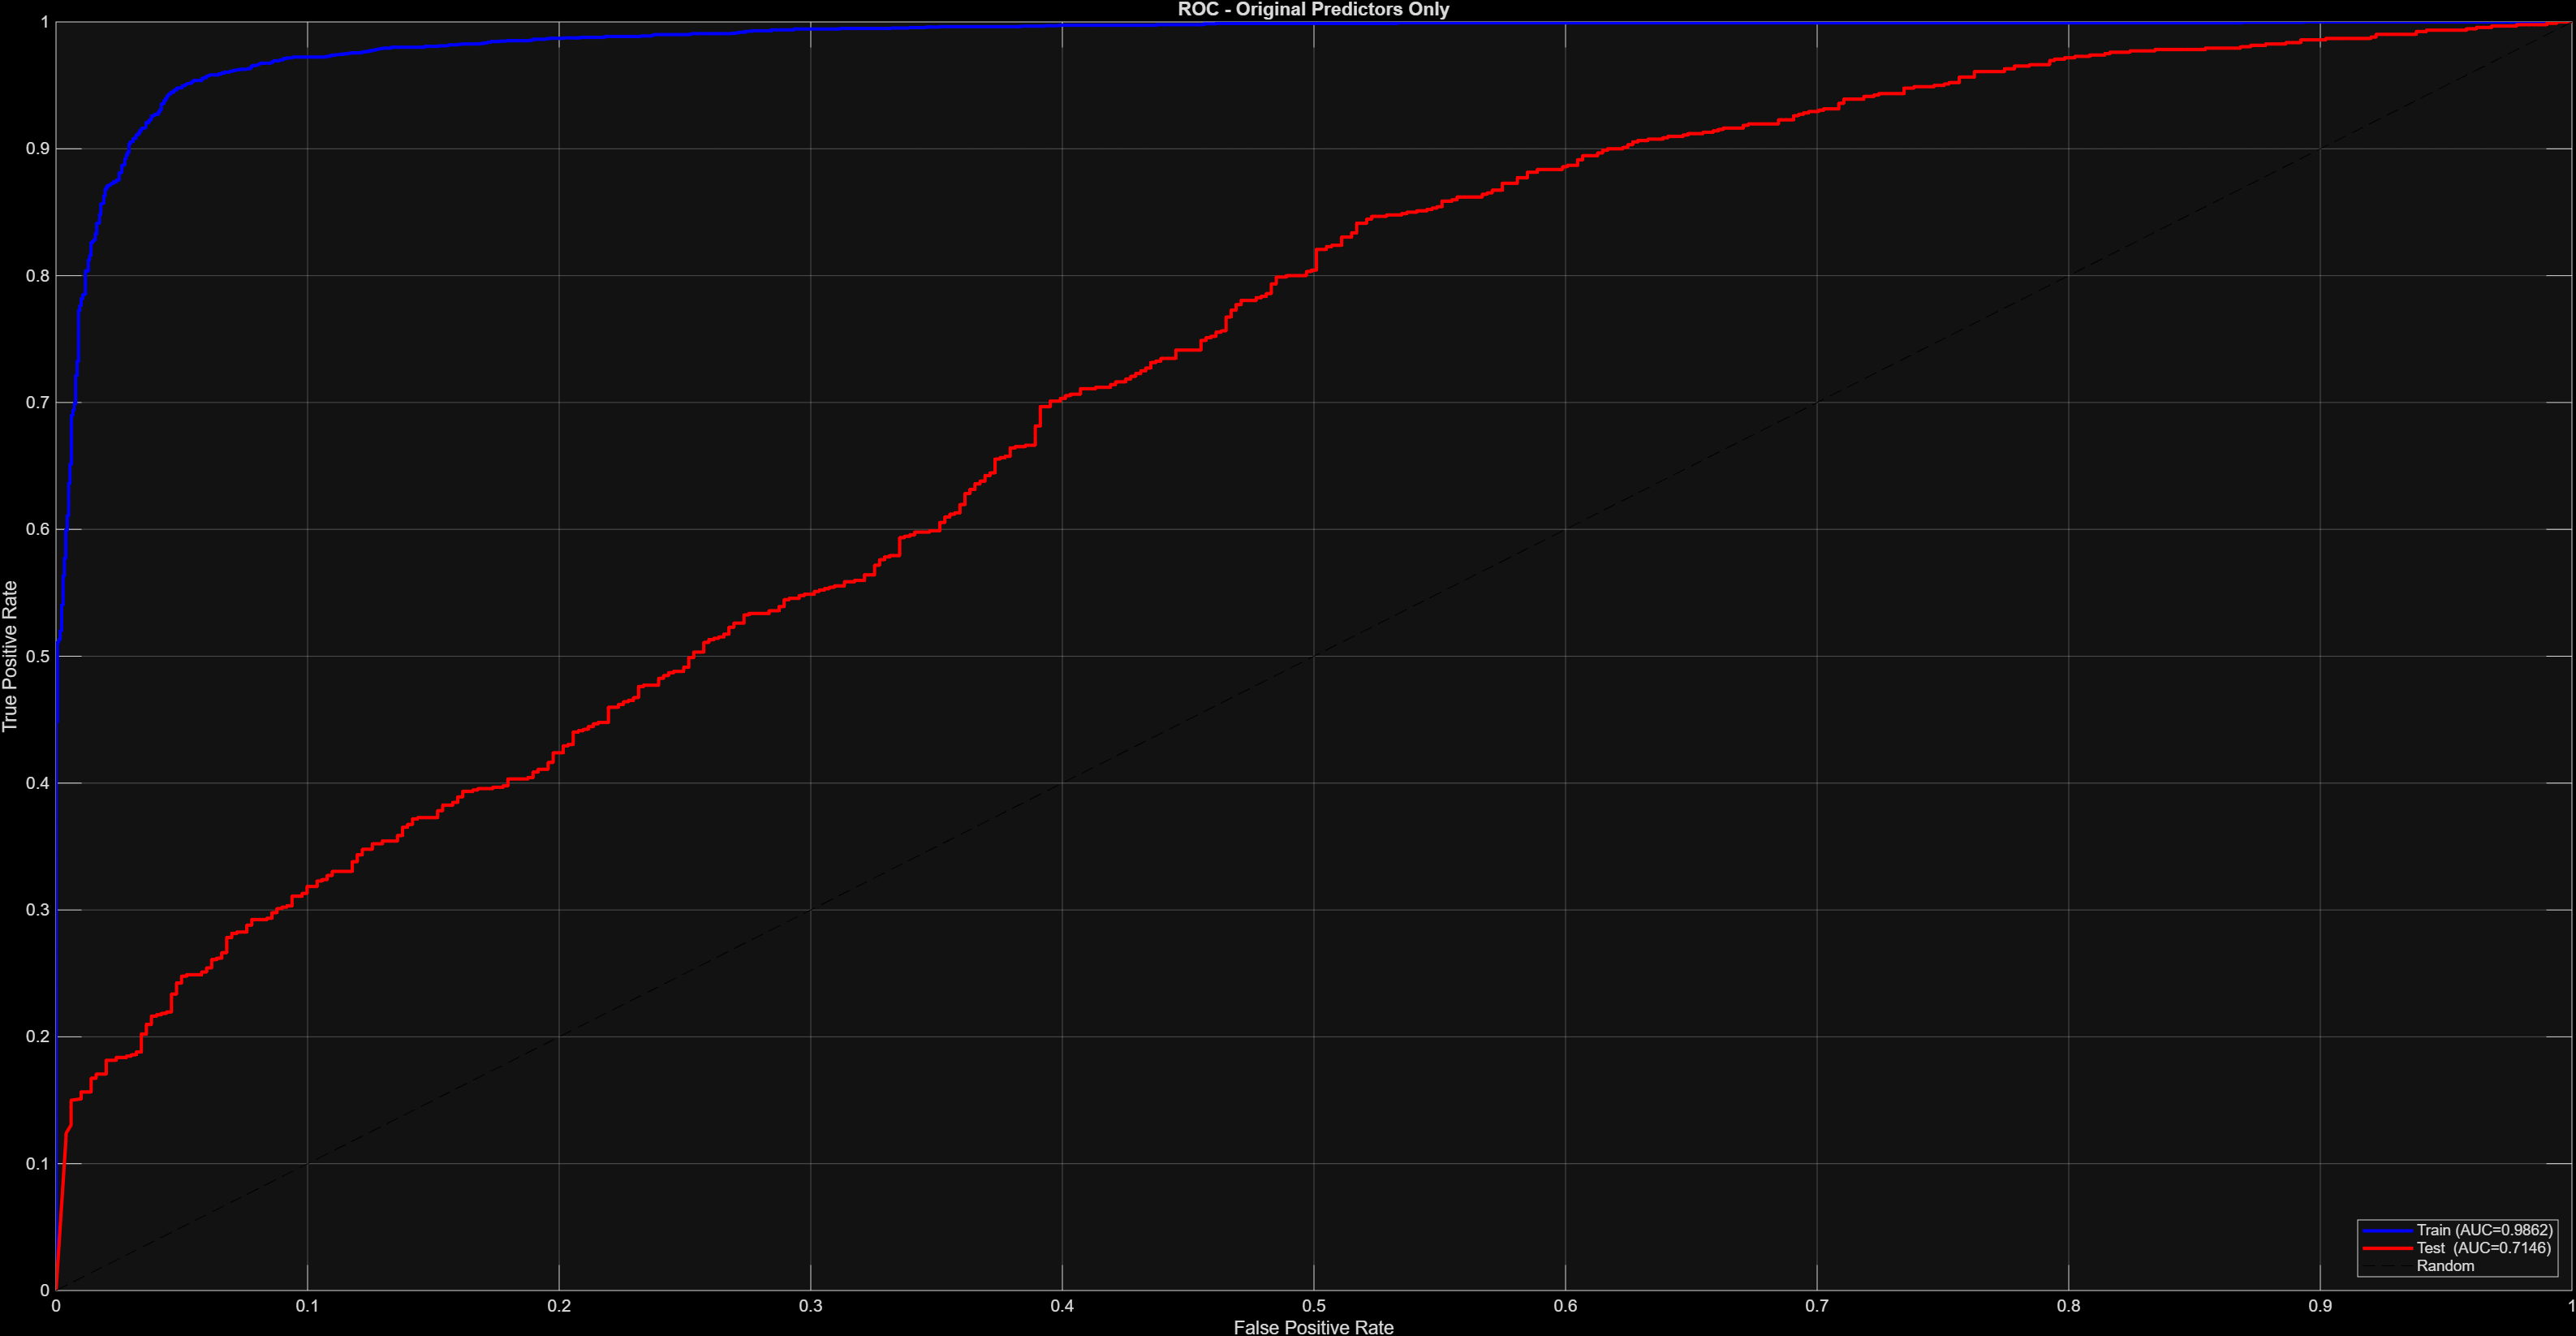
\includegraphics[width=0.75\textwidth]{Figs/ROC - Original Predictors Only.png}
		\caption{ROC curves using only the original 923 predictors. The blue curve (training, AUC = 0.9862) hugs the upper-left corner, while the red curve (test, AUC = 0.7146) shows much weaker discrimination.}\label{fig:roc_orig}
	\end{figure}

	\newpage
	%----------------------------------------------------------------------
	\subsection{Combined Predictors: Original + Change Rate (1{,}846 Features)}
	%----------------------------------------------------------------------

	Adding the 923 change rate columns doubles the feature count to 1{,}846. The logistic regression results are shown in Figure~\ref{fig:roc_comb}.

	\begin{table}[H]
		\centering
		\caption{AUC results with combined predictors (original + change rate).}\label{tab:auc_comb}
		\begin{tabular}{lc}
			\toprule
			\textbf{Dataset} & \textbf{AUC} \\
			\midrule
			Training & 1.0000 \\
			Test     & 0.6463 \\
			\bottomrule
		\end{tabular}
	\end{table}

	With 1{,}846 features (more than one-third the number of training samples), the model achieves perfect separation on the training set (AUC = 1.0), accompanied by MATLAB's warning about perfect separation. However, test AUC \textit{decreases} from 0.7146 to 0.6463. This is a clear demonstration that naively adding more features without selection worsens overfitting and degrades generalization performance.

	\begin{figure}[H]
		\centering
		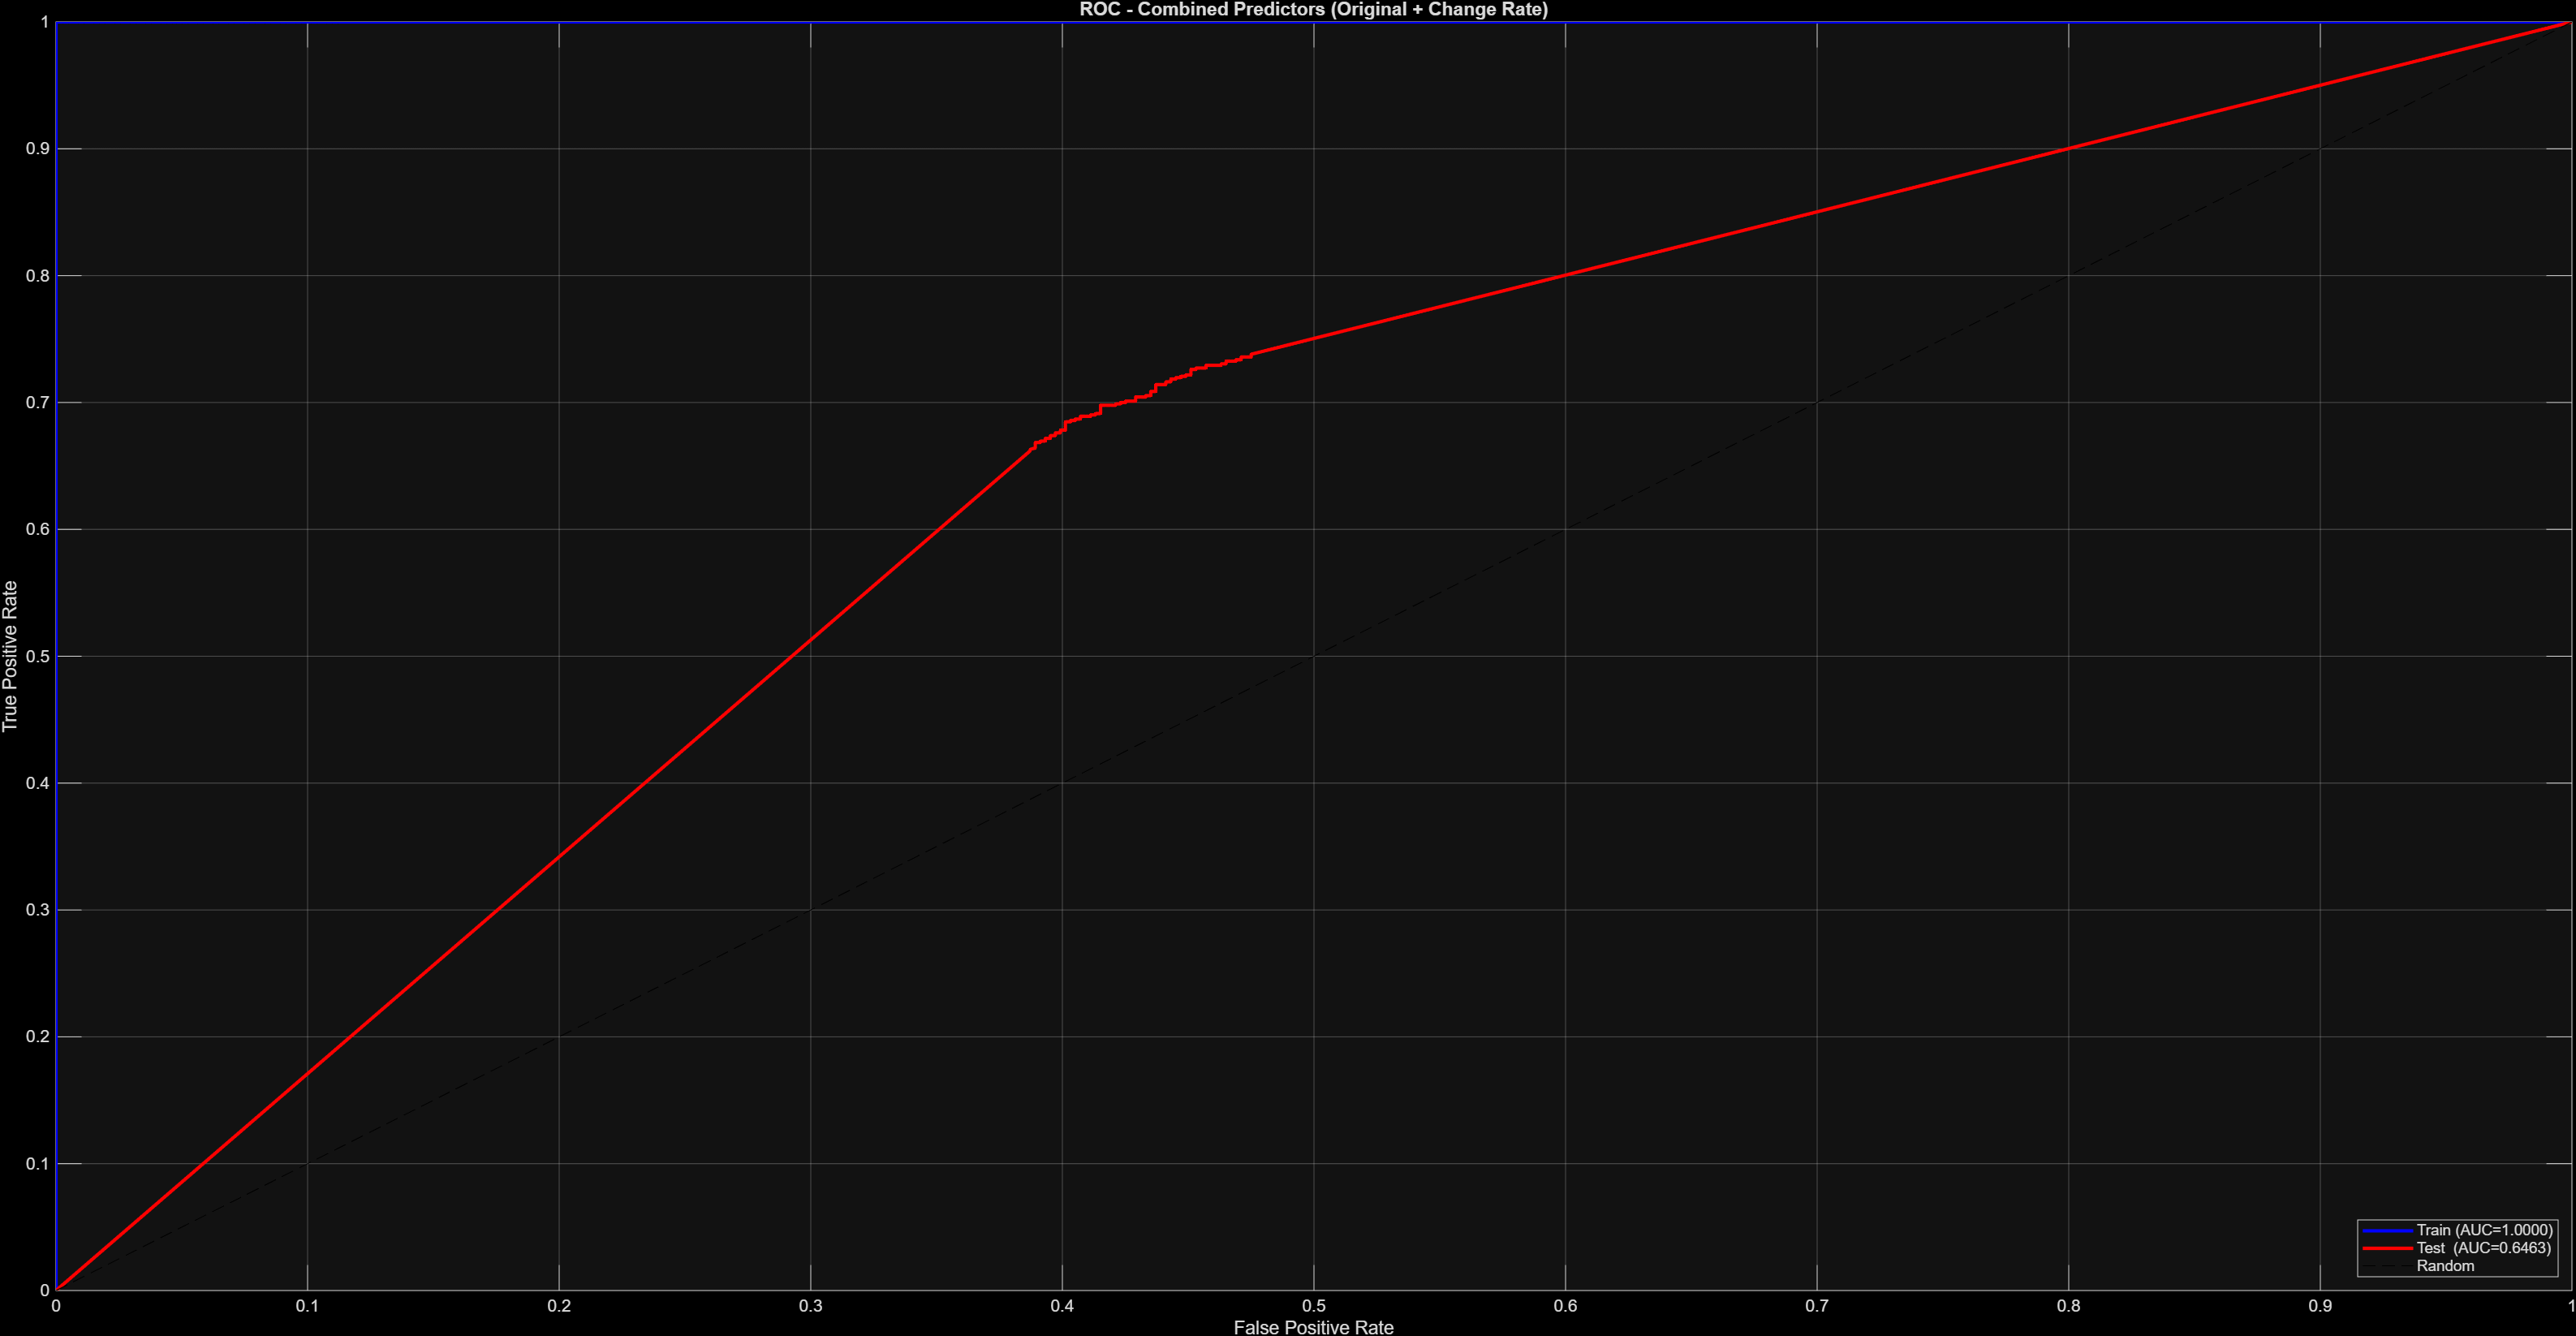
\includegraphics[width=0.75\textwidth]{Figs/ROC - Combined Predictors (Original + Change Rate).png}
		\caption{ROC curves using all 1{,}846 combined predictors. The training ROC (blue, AUC = 1.0) is a flat line along the top, indicating perfect separation. The test ROC (red, AUC = 0.6463) is nearly diagonal, showing poor generalization.}\label{fig:roc_comb}
	\end{figure}

	\newpage
	%======================================================================
	\section{Step 3: Feature Selection}\label{sec:featsel}
	%======================================================================

	The \texttt{featureSelection.m} function (which uses MATLAB's \texttt{sequentialfs} with the \texttt{critfun.m} criterion function) was applied to the combined 1{,}846-feature training set. This function performs \textbf{sequential forward selection}: starting from an empty set, it greedily adds the feature that most reduces the binomial deviance at each step. It stops when no remaining feature can reduce deviance by more than $\chi^{2}_{0.95,1} \approx 3.84$.

	\subsection{Results}

	The algorithm selected \textbf{162 features} over 163 steps:

	\begin{itemize}
		\item \textbf{96 features} from the original predictor columns (indices $\leq$ 923)
		\item \textbf{66 features} from the change rate columns (indices $>$ 923)
	\end{itemize}

	This result demonstrates that the newly generated change rate predictors \textbf{do have a meaningful impact on feature selection}. Approximately 41\% of the selected features (66 out of 162) come from the change rate matrix, confirming that daily change rate captures predictive information not already present in the raw values alone.

	\subsection{Observations on the Selection Order}

	The first feature added (column 349) produced the largest single deviance reduction, from 6{,}050.37 down to 3{,}664.07 --- a drop of 2{,}386.3. The first change rate feature to enter was column 1{,}696 (original column 773's change rate) at step 11, relatively early in the process. This further confirms that change rate features carry meaningful signal.

	\newpage
	%======================================================================
	\section{Step 4: AUC vs.\ Number of Top Selected Features}\label{sec:topk}
	%======================================================================

	To observe how different numbers of features affect AUC, the features were ranked by individual deviance (lower deviance = more predictive). Logistic regression was then fit using the top $K$ features for $K \in \{5, 10, 15, 20, 25, 30, 50\}$.

	\begin{table}[H]
		\centering
		\caption{Training and test AUC as a function of the number of top-ranked features used.}\label{tab:topk}
		\begin{tabular}{ccc}
			\toprule
			\textbf{Top $K$ Features} & \textbf{Training AUC} & \textbf{Test AUC} \\
			\midrule
			5  & 0.9045 & \textbf{0.8890} \\
			10 & 0.9047 & 0.8889 \\
			15 & 0.9057 & 0.8878 \\
			20 & 0.9063 & 0.8873 \\
			25 & 0.9076 & 0.8837 \\
			30 & 0.9080 & 0.8841 \\
			50 & 0.9093 & 0.8838 \\
			\midrule
			923 (original only) & 0.9862 & 0.7146 \\
			1{,}846 (all combined) & 1.0000 & 0.6463 \\
			\bottomrule
		\end{tabular}
	\end{table}

	\begin{figure}[H]
		\centering
		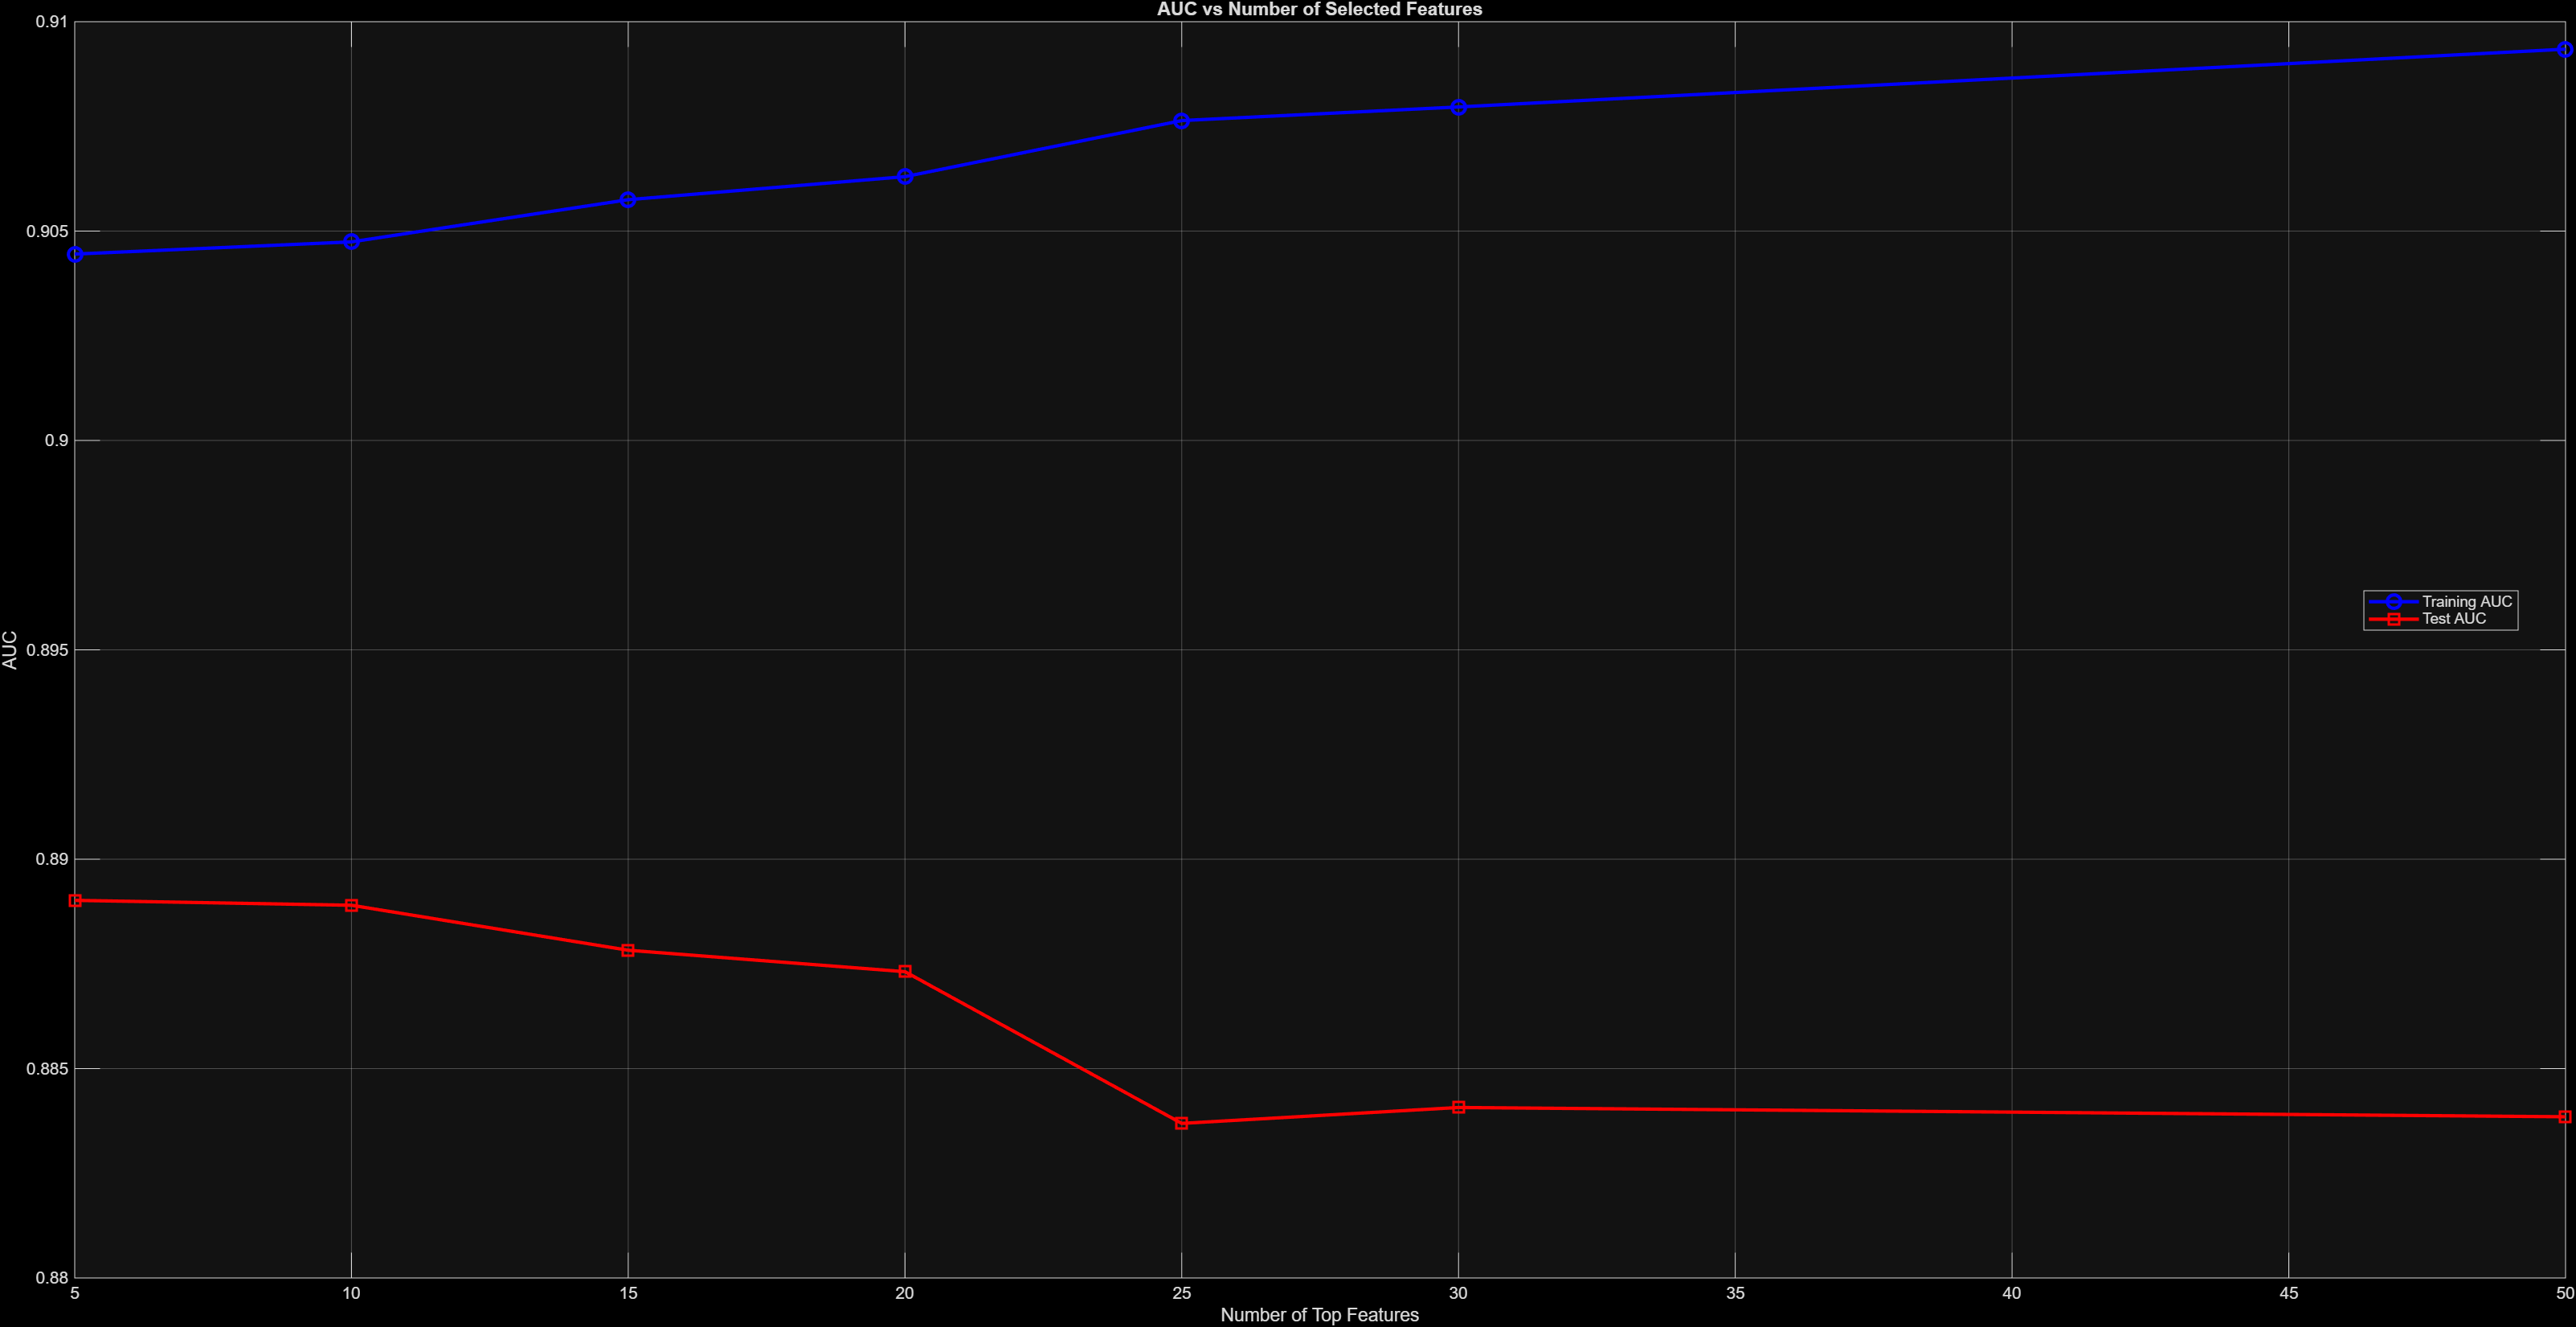
\includegraphics[width=0.75\textwidth]{Figs/AUC vs Number of Selected Features.png}
		\caption{AUC vs.\ number of top-ranked features. Training AUC (blue) increases monotonically with more features, while test AUC (red) is highest at $K = 5$ and gradually decreases.}\label{fig:auc_vs_k}
	\end{figure}

	\subsection{Key Observations}

	\begin{enumerate}
		\item \textbf{Feature selection dramatically improves test AUC.} Using just the top 5 features yields a test AUC of 0.889, compared to 0.715 with all 923 original features and 0.646 with all 1{,}846 combined features.

		\item \textbf{The best test AUC occurs with the fewest features ($K = 5$).} The test AUC values are remarkably stable across all values of $K$ tested (ranging from 0.884 to 0.889), but the slight downward trend shows that adding more features provides diminishing returns on the test set while increasing overfitting risk.

		\item \textbf{Training AUC increases monotonically with $K$}, which is expected --- more features always allow the model to fit the training data more closely. But this does not translate to better generalization.

		\item \textbf{The train--test gap grows with more features.} At $K = 5$, the gap is only $0.905 - 0.889 = 0.016$. At $K = 50$, it grows to $0.909 - 0.884 = 0.025$. With all 1{,}846 features, the gap is $1.000 - 0.646 = 0.354$.
	\end{enumerate}

	\newpage
	%======================================================================
	\section{Step 5: Test ROC Curves for Different Feature Subsets}
	%======================================================================

	Figure~\ref{fig:roc_subsets} overlays the test-set ROC curves for each value of $K$. All curves are tightly clustered near each other, reflecting the similar test AUC values observed in Table~\ref{tab:topk}.

	\begin{figure}[H]
		\centering
		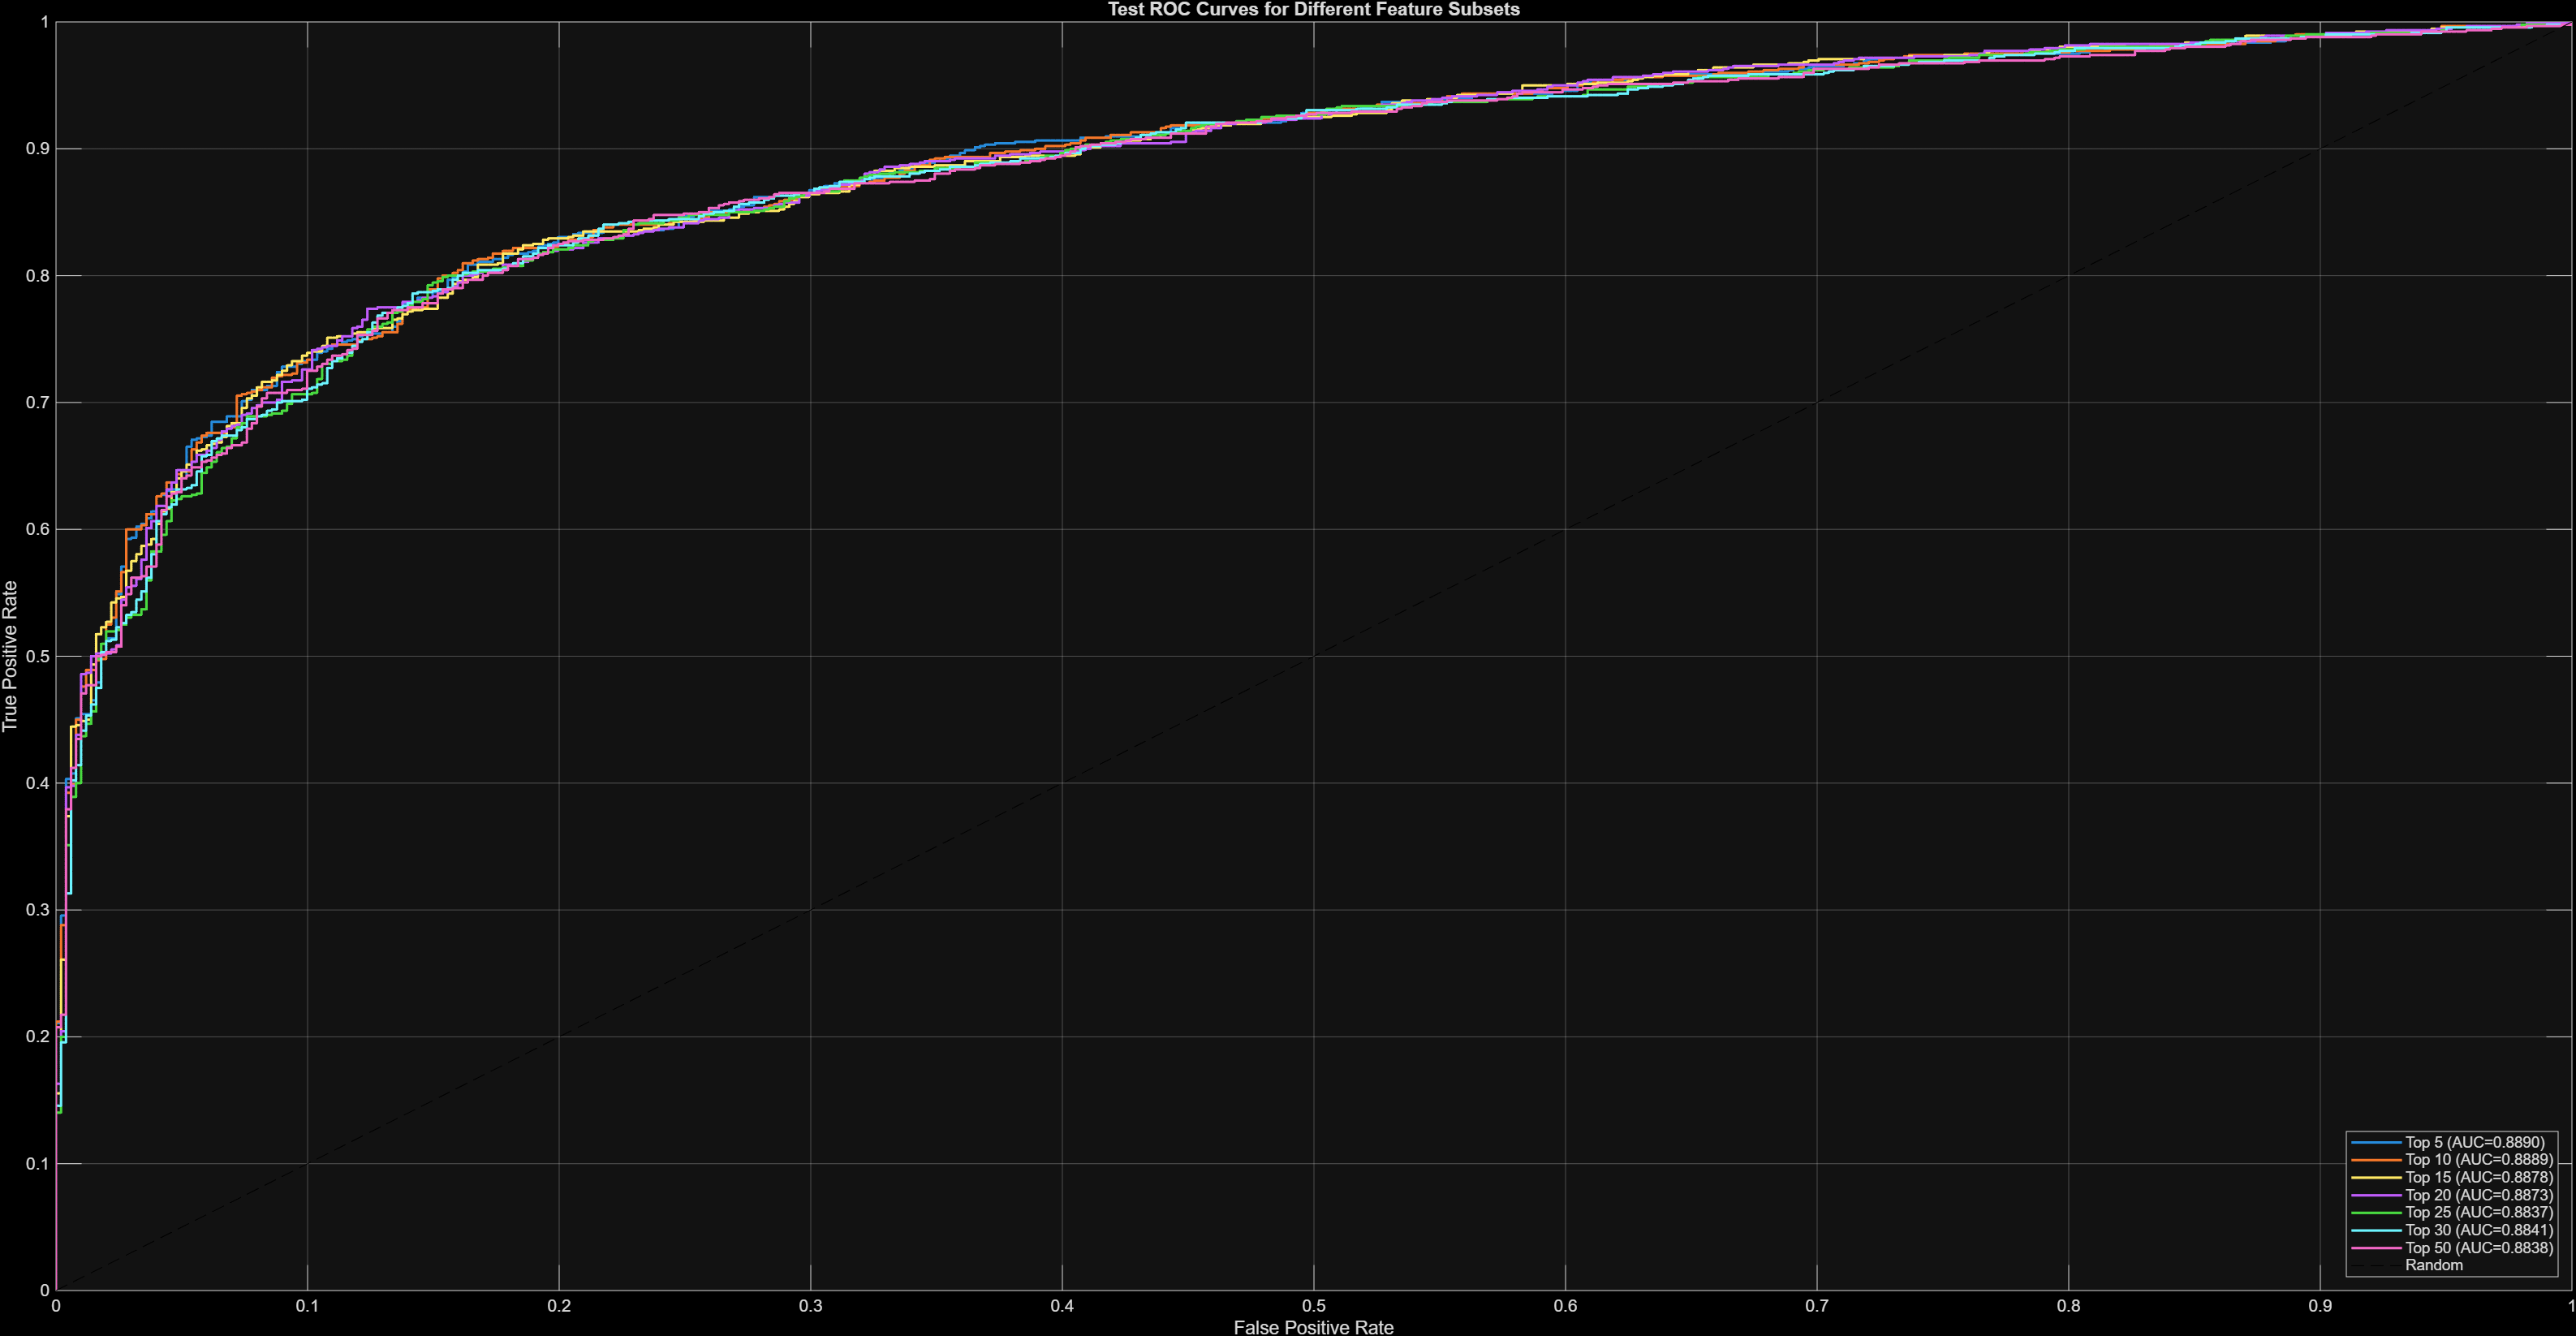
\includegraphics[width=0.75\textwidth]{Figs/Test ROC Curves for Different Feature Subsets.png}
		\caption{Test ROC curves for different numbers of top-ranked features. All subsets achieve similar test performance (AUC $\approx$ 0.884--0.889), confirming that a small number of well-chosen features is sufficient.}\label{fig:roc_subsets}
	\end{figure}

	\newpage
	%======================================================================
	\section{Conclusion}
	%======================================================================

	\begin{enumerate}
		\item \textbf{Adding the change rate predictors impacts feature selection.} Of the 162 features selected by sequential forward selection, 66 (41\%) came from the change rate matrix. The change rate features capture temporal dynamics (rate of change between consecutive time steps) that complement the raw predictor values.

		\item \textbf{Blindly adding more features hurts generalization.} Doubling the feature count from 923 to 1{,}846 reduced the test AUC from 0.715 to 0.646, while inflating training AUC to a perfect 1.0. This demonstrates the curse of dimensionality and the danger of overfitting when features outnumber the signal.

		\item \textbf{Feature selection is essential.} Selecting a small subset of the most informative features improved test AUC from 0.646 (all features) to 0.889 (top 5 features) --- a dramatic improvement. The top 5 features alone outperform models using 10$\times$ to 370$\times$ as many features.

		\item \textbf{Diminishing returns beyond a handful of features.} Test AUC is nearly flat across $K = 5$ to $K = 50$, suggesting that the bulk of the predictive signal is concentrated in very few features and that additional features contribute primarily noise.
	\end{enumerate}

	\newpage
	%======================================================================
	\section{Appendix: MATLAB Code}
	%======================================================================

	\lstinputlisting[caption={EE627\_HW6\_Echete.m --- Main homework script},label={lst:main}]{EE627_HW6_Echete.m}
    \newpage
	\vspace{1em}

	\lstinputlisting[caption={featureSelection.m --- Sequential forward feature selection wrapper},label={lst:feaSel}]{featureSelection.m}

	\vspace{1em}

	\lstinputlisting[caption={critfun.m --- Criterion function (binomial deviance)},label={lst:critfun}]{critfun.m}

	\newpage
	%======================================================================
	\section{Appendix: Console Output}
	%======================================================================

	\lstinputlisting[caption={Results.txt --- Full MATLAB console output},label={lst:results},language={},keywordstyle=\ttfamily,stringstyle=\ttfamily]{Results.txt}

\end{document}
